\subsection{极限定理}
\subsubsection{更新过程的大数定律}

先讲一下过程本身的极限.
\begin{lemma}\label{lem:p114-lem2}
    \[
    N(t)\as{t} +\infty
    \]
    即存在零测集 $\tilde{\Omega}^c,\stt \forall \omega \in \tilde{\Omega}$, 有 $\lim_{t\to\infty}N(t)(\omega)=+\infty$. 即 $\PP(\lim_{t\to\infty}N(t)=+\infty)=1$.

    注: $N(t)$ 非可列 r.v., 但 $\lim_{t\to\infty}N(t)$ 仍为 r.v., 因为 $N(t)$ 关于 $t$ 右连左极 (\textit{cadlag}), 即右连续存在, 左极限存在.
\end{lemma}

\begin{proof}
    $\lim_{t\to\infty}N(t)<+\infty$, $N(t)$关于$t\uparrow$ 单调上升.

    $\Rightarrow \exists M>0,\stt \forall t\geq 0, N(t)\leq M\Rightarrow T_M\leq t< T_{M+1}$

    $\Rightarrow \forall t\geq 0,T_{M+1}>t$

    $\Rightarrow T_{M+1}=+\infty$
    \[
    \begin{aligned}
        \PP(\limit{t}N(t)<+\infty)&\leq \PP(\exists n,T_n=+\infty)=\PP(\exists n,\tau_n=+\infty)\\
        &\leq \sum_{n\geq 1}\PP(\tau_n=+\infty)=\sum_{n\geq 1}(1-\PP(\tau_n<+\infty))\\
        &=\sum_{n\geq 1}(1-\limit{t_n}F(t_n))=0
    \end{aligned}
    \]
\end{proof}

\begin{theorem}[更新过程的LLN]\label{thm:p114-thm3.1}
    \[
    \frac{N(t)}{t}\as{t}\frac{1}{\EE\tau_1}
    \]
    即 $\displaystyle\PP(\limit{t}\frac{N(t)}{t}=\frac{1}{\EE\tau_1})=1$, (因$\displaystyle\frac{N(t)}{t}$ cadlag). 
\end{theorem}

\begin{proof}
    当$N(t)<+\infty$时, $T_{N(t)}\leq t<T_{N(t)+1}$

    当$0<N(t)<+\infty$时,
    \[
    \begin{aligned}
        \boxed{\frac{T_{N(t)}}{N(t)}}\leq \frac{t}{N(t)}&<\frac{T_{N(t)+1}}{N(t)}\\
        &=\boxed{\frac{T_{N(t)+1}}{N(t+1)}}\cdot \frac{N(t+1)}{N(t)}
    \end{aligned}
    \tag{*1}
    \]
    方框内极限相同.
    \begin{enumerate}
        \item 由 Lem \ref{lem:p114-lem2} 知, $\exists \tilde{\Omega}_1^c,\PP(\tilde{\Omega}_1^c)=0,\stt \forall \omega\in \tilde{\Omega}_1, \limit{t}N(t)(\omega)=+\infty$.
        \[
        \omega\in\tilde{\Omega}_1,\limit{t}\frac{N(t)+1}{N(t)}(\omega)=1
        \]
        \item 由 SLLN 知, $\frac{1}{n}T_n\as{n}\EE\tau_1$
        
        $\Rightarrow \exists \tilde{\Omega}_2^c, \PP(\tilde{\Omega}_2^c)=0,\stt \forall \omega\in\tilde{\Omega}_2, \limit{n}\frac{T_n}{n}(\omega)=\EE\tau_1$

        $\Rightarrow \forall \omega\in\tilde{\Omega}_1\cap \tilde{\Omega}_2=(\tilde{\Omega}_1^c\cup \tilde{\Omega}_2^c)^c$, 有
        \[
        \limit{t}\frac{T_{N(t)}}{N(t)}(\omega)=\EE\tau_1
        \]
        (这里用$\epsilon-\delta$语言自己写一下)
    \end{enumerate}
    由 1, 2, (*1) 知, $\frac{t}{N(t)}\as{t}\EE\tau_1$.
\end{proof}

\subsubsection{更新报酬过程及LLN}

\begin{definition}
    设 $\{N(t),t\geq 0\}$ 为一更新过程. $\{\tau_k, k\geq 1\}$ 为其时间间隔序列, 设 $\{r_k,k\geq 1\}$ 为一 iid 随机变量列, 则称由 $R(t):=\sum_{k=1}^{N(t)}r_k$ 定义的过程 $\{R(t),t\geq 0\}$ 为更新报酬过程.
\end{definition}
注:
\begin{enumerate}
    \item $r_k$: 第$k$次更新时刻 ($T_k$) 的报酬/花费
    \item $R(t)$: $[0,t]$中总报酬 ($[0,T_{N(t)}]$, 忽略 $(T_{N(t)},t]$).
\end{enumerate}

\begin{theorem}[更新报酬过程的LLN]\label{thm:p116-thm3.3}
    设 $\EE|r_1|<\infty,\EE|\tau_1|\in (0,+\infty)$, 则
    \[
    \frac{R(t)}{t}\as{t}\frac{\EE r_1}{\EE\tau_1}
    \]
\end{theorem}

\begin{proof}
    \[
    \frac{R(t)}{t}=\frac{\sum_{k=1}^{N(t)}r_k}{N(t)}\cdot\frac{N(t)}{t}
    \tag{*}
    \]
    \begin{enumerate}
        \item 由 SLLN 知, \framebox{$\frac{1}{n}\sum_{k=1}^n r_k$}$\as{n}\EE r_1$. 又 Lem \ref{lem:p114-lem2} 知, \framebox{$N(t)$}$\as{t}+\infty$. 所以 $\sum_{k=1}^{N(t)} r_k/N(t)\as{t}\EE r_1$
        \item 由 Thm \ref{thm:p114-thm3.1} 知, 
        \[
        \frac{N(t)}{t}\as{t}\frac{1}{\EE \tau_1}
        \]
    \end{enumerate}
    由 1, 2, (*) 知
    \[
    \frac{R(t)}{t}\as{t}\frac{\EE r_1}{\EE\tau_1}
    \]
\end{proof}

\begin{example}[长远看汽车的费用]
    1. 一辆车的寿命 (首次发生故障的事件) $X_k$: 密度函数 $h$, $\{X_k,k\geq 1\}$ iid

    2. 更新间隔时间 (买新车): $\tau_k=X_k\land T$

    3. 第$k$次更新产生的花费: $r_k=A(\text{买新车})+B\II_{\{\tau_k\leq T\}}$

    问: 长远来看, 单位时间的花费是多少? (用LLN)
\end{example}
\[
\frac{\sum_{k=1}^{N(t)}r_k}{t}\leq \frac{[0,t]\text{间的花费}}{t}\leq \frac{\sum_{k=1}^{N(t)+1}r_k}{t}
\]
从左到右分别对应时间 $[0,T_{N(t)}],[0,t],[0,T_{N(t)+1}]$

\begin{proof}[解]
    令 $R(t):=\sum_{k=1}^{N(t)}r_k$, 其中 $N(t)=\max\{n|\sum_{k=1}^n\tau_k\leq t\}$ (买新车的更新过程). 欲求 $\limit{t}\frac{R(t)}{t}$.
    \[
    \begin{aligned}
        \EE\tau_1=\EE(X_1\land T)&=\int_0^{+\infty}(x\land T)h(x)dx\\
        &=\int_0^T xh(x)dx+\int_T^{+\infty}T h(x)dx
    \end{aligned}
    \]
    \[
    \EE r_1 =A+B\EE \II_{\{\tau_1<T\}}=A+B\EE \II_{\{X_1<T\}}=A+B\int_0^T h(x)dx
    \]
    由 Thm \ref{thm:p116-thm3.3} 知,
    \[
    \limit{t}\frac{R(t)}{t}=\frac{A+B\int_0^T h(x)dx}{\int_0^{+\infty}(x\land T)h(x)dx}, \text{a.s.}
    \]
\end{proof}

\begin{theorem}[Ross, Thm 3.6.1]
    设 $\{(r_k,\tau_k),k\geq 1\}$ 是 iid 的,
    \[
    \limit{t}\frac{\EE R(t)}{t}=\frac{\EE r_1}{\EE\tau_1}
    \]
    LHS是数的极限, 不是随机变量的极限. 其中 $\frac{\EE R(t)}{t}$ 被称为更新报酬函数.
\end{theorem}
注: $\{(\tau_k,r_k),k\geq 1\}$ 相互独立 $\Rightarrow$
    \begin{enumerate}
        \item $\{\tau_k,k\geq 1\}$ 相互独立, $\{r_k,k\geq 1\}$ 相互独立
        \item $\{\tau_k,1\leq k\leq n\}\ind \{r_k,k\geq n+1\}$
        \item $\{\tau_k\}\ind \{r_j,j\neq k\}$ ($r_k$取全集即可)
    \end{enumerate}

\subsubsection{交替更新过程及LLN}

\begin{definition}
    设 $\{(s_k,u_k),k\geq 1\}$ 为 iid 的随机变量向量列, $s_k\geq 0,u_k\geq 0,\forall k\geq 1$. 令 $\tau_k:=s_k+u_k,k\geq 1$. 定义
    \[
    N(t)=\begin{cases}
        \max\{n|\sum_{k=1}^n\tau_k\leq t\} & t>0\\
        0 & t=0
    \end{cases}
    \]
    称 $\{N(t),t\geq 0\}$ 为交替更新过程.
\end{definition}

\begin{theorem}[交替更新过程的LLN]\label{thm:p118-thm3.4}
    设存在分布函数 $H$ 使得 $\tau_k\sim H, \EE s_1\in (0,+\infty), \EE u_1\in (0,+\infty)$, 则
    \begin{enumerate}
        \item $\displaystyle \frac{\sum_{k=1}^{N(t)}s_k}{t}\as{t}\frac{\EE s_1}{\EE s_1+\EE u_1}$
        \item $\displaystyle \frac{[0,t]\text{中系统处于状态1的时长}}{t}\as{t}\frac{\EE s_1}{\EE s_1+\EE u_1}$, 即系统处于状态1的事件比例的极限为 $\displaystyle\frac{\EE s_1}{\EE s_1+\EE u_1}$
    \end{enumerate}
\end{theorem}

\begin{proof}
    \begin{enumerate}
        \item Thm \ref{thm:p116-thm3.3} 中取 $r_k=s_k$.
        \item 令 $U(t):=[0,t]$ 中系统处于状态1的时长
        \[
        \frac{\sum_{k=1}^{N(t)}s_k}{t}\leq \frac{u(t)}{t}\leq \frac{\sum_{k=1}^{N(t)+1}s_k}{t}=\frac{\sum_{k=1}^{N(t)+1}s_k}{N(t)+1}\cdot\frac{N(t)+1}{N(t)}
        \]
        由 Thm \ref{thm:p116-thm3.3} 得到想要的结果.
    \end{enumerate}
\end{proof}

\subsubsection{使用年龄和剩余寿命}

\begin{figure}[H]
    \centering
    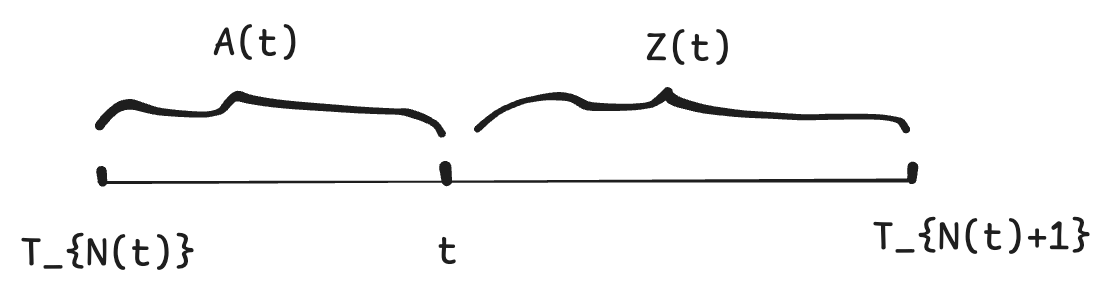
\includegraphics[width=0.55\textwidth]{figures/p119.png}
\end{figure}

$A(t)$ 为使用年龄, $A(t)=t-T_{N(t)}$. $Z(t)$ 为剩余寿命, $Z(t)=T_{N(t)+1}-t$.

\begin{example}
    某零件按更新过程 $\{N(t),t\geq 0\}$ 替换, 其更新间隔时间序列 $\{\tau_k,k\geq 1\}$. 设 $\EE \tau_1^2<\infty$, 且 $0<\EE\tau_1<\infty$, 则零件的长程平均使用年龄
    \[
    \limit{t}\frac{1}{t}\int_0^tA(s)ds=\frac{\EE\tau_1^2}{2\EE\tau_1}
    \]
    若是长程平均寿命即把 $A(s)$ 换成 $Z(s)$.
\end{example}
注: $\int_0^tA(s)ds$有无意义? 有的, 因为 $N(t)$ 是几乎处处右连左极, 在 $[0,t]$ 内有有限多跳. 并非闭区间内的连续函数才可积 (参考梅加强\cite{jiaqiang}).
\begin{figure}[H]
\centering
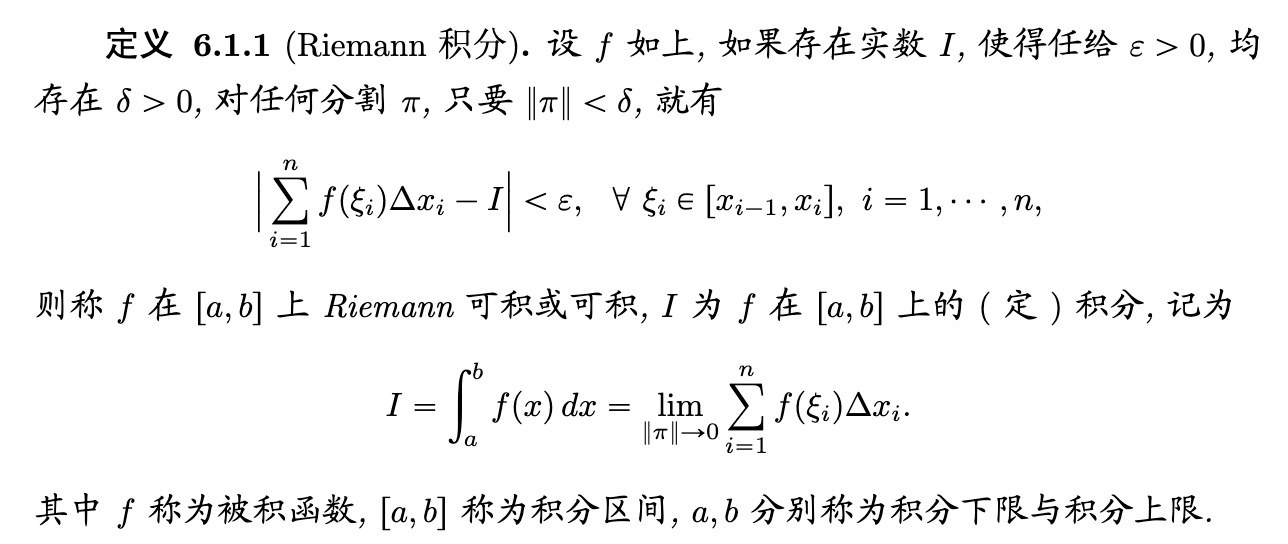
\includegraphics[width=0.75\textwidth]{figures/Riemann-integral.png}
\caption{定义6.1.1-Riemann积分}
\end{figure}

\begin{proof}
    由 $T_{N(t)}\leq t$,
    \[
    \begin{aligned}
        \int_0^t A(s)ds &\geq \int_0^{T_{N(t)}}A(s)ds\\
        &=\sum_{k=1}^{N(t)}\int_{T_{k-1}}^{T_k}(s-T_{N(s)})ds\\
        &=\sum_{k=1}^{N(t)}\int_{T_{k-1}}^{T_k}(s-T_{k-1})ds\\
        &=\sum_{k=1}^{N(t)}\frac{1}{2}(s-T_{k-1})^2\bigg|_{T_{k-1}}^{T_k}\\
        &=\sum_{k=1}^{N(t)}\frac{1}{2}(T_k-T_{k-1})^2=\frac{1}{2}\sum_{k=1}^{N(t)}\tau_k^2
    \end{aligned}
    \]
    由 Thm \ref{thm:p116-thm3.3} 知,
    \[
    \frac{1}{2t}\sum_{k=1}^{N(t)}\tau_k^2\as{t}\frac{\EE \tau_1^2}{2\EE\tau_1}
    \]
    同理,
    \[
    \begin{aligned}
        \int_0^t A(s)ds &\leq \int_0^{T_{N(t)+1}} A(s)ds\\
        &=\sum_{k=1}^{N(t)+1}\frac{1}{2}(T_k-T_{k-1})^2\\
        &=\frac{1}{2}\sum_{k=1}^{N(t)+1}\tau_k^2
    \end{aligned}
    \]
    由 Thm \ref{thm:p116-thm3.3} 知,
    \[
        \frac{1}{2t}\sum_{k=1}^{N(t)}\tau_k^2\as{t}\frac{\EE \tau_1^2}{2\EE\tau_1}
    \]
\end{proof}
\newpage